\subsection{Chess}
Chess is a board game of two oppenent players. It's a turn-based game which means one player makes a move, 
then the other player makes a move, then the first player makes a move and so on. Chess is played on a board of $8 \times 8$ squares. The squares are typically black and white, but can be any two colors (see figure \ref{fig:chess}). The squares can only contain one piece at a time, unlike games like Mancala and Backgammon. Each player has a total of 16 pieces: 8 pawns, 2 knights, 2 bishops, 2 rooks, a queen and a king. Each type of piece has unique ways to move. For instance a pawn can move only one square vertically forward or one square diagonal when capturing an enemy piece. A rook can move unlimited squares either forward or backward (vertical movement), or to the right or to the left (horisontal movement). This separates it's pieces from a lot of other board games where all pieces have the same abilities e.g. Naughts and Crosses, Mancala, Ludo, Backgammon etc.  

Cut to the bone the game goes as follow: When a game starts the pieces are in their respective starting positions as seen in figure \ref{fig:chess}. The player with the white pieces always makes the first move, and after that the players shifts in turn in which clever moves are beeing taken and pieces are beeing captured until one player has checkmated the other - and the game is over. The checkmate situation is obtained when the king piece is in a position to be captured and cannot escape from capture. \cite{chessrules}.

Special situation and moves. In chess there are numerus special situations and moves which doesn't follow the normal pattern of chess. Earlier we mentioned that a pawn can only move only one square vertically forward or one square diagonal when capturing an enemy piece. But this is not always true. If the pawn is in it's respective starting position it can move either one \textbf{or} two squares vertically forward. After moving from it's starting position it can only move one square forward the rest of the game. Another special move is the move called ``castling''. This move allows a player to move two pieces in one turn (the king and one of the rooks). But to do the move several conditions needs to be met. First: the move has to be the very first move of the king and the rook, second: there can't be any pieces standing between the king and the rook and third: there can't be any opposing pieces that could capture the king in his original square, the squares he moves through or the square he end up in \cite{chessrules}.

\begin{figure}
	\centering
		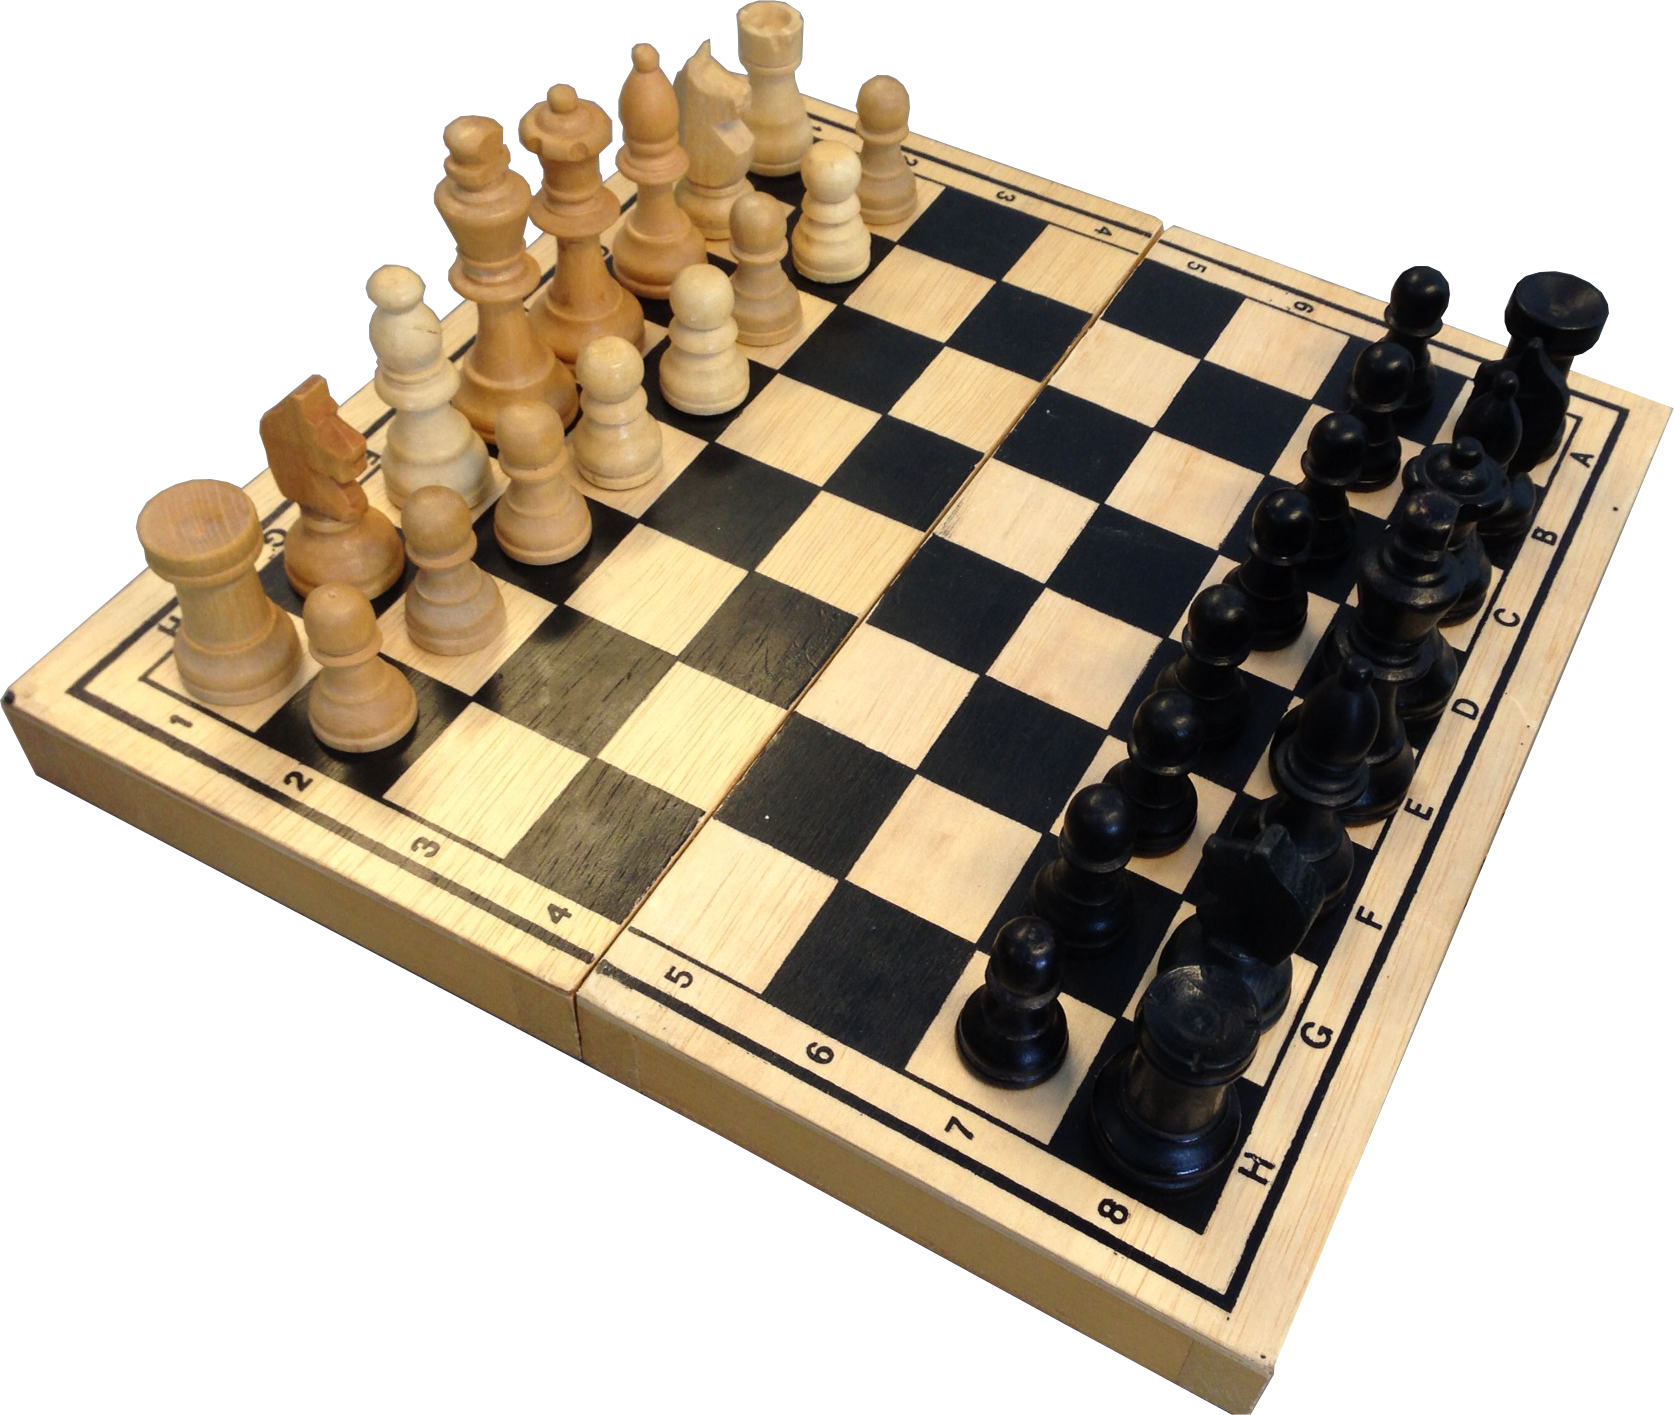
\includegraphics[scale=0.1]{pictures/chess.png}
		\capt{The board game chess with the pieces in start position.}
\label{fig:chess}
\end{figure}

Possible requirements
\begin{itemize}[noitemsep]
\item pieces with different movement abilities.
\item A square board with a number of squares in it.
\item A winning condition - when the king has been checkmated.
\item A starting state - how the pieces are placed on the board before the game's very first move.
\item Defining special situations like the ``castling''
\end{itemize}